\documentclass[times, % the default MS fonts which the commission likes
               specification,annotation, % generate aux pages in the primary language
               titlepage-extra-ru,specification-extra-ru,annotation-extra-ru, % generate aux pages + title in Russian
               languages={russian,english} % sets English as the primary language and also loads Russian
              ]{itmo-student-thesis}

%% Package options:
%% - times:          uses the Microsoft "corefonts" for everything, uses xelatex
%% - specification:  when present, generates the "objectives" page, aka specification, in primary language, which is English in this example
%% - annotation:     when present, generates the "summary" page, aka annotation, in primary language, which is English in this example
%% - titlepage-extra-ru:     when present, generates the title page in Russian
%% - specification-extra-ru: when present, generates the "objectives" page, aka specification, in Russian
%% - annotation-extra-ru:    when present, generates the "summary" page, aka annotation, in Russian
%% - languages={...}: sets the languages used in this document.
%%                    This is passed directly to babel. If it is just the comma-separated list of languages, the last language becomes the primary one.
%%                    It must include Russian at least to generate "extra-ru" pages, although not including it may break things.

%% The packages and \begin{filecontents}...\end{filecontents} are for illustrative purposes only.
%% Instead of filecontents, please consider using a normal bibliography file.
\usepackage{tikz}
\usetikzlibrary{arrows}
\usepackage{filecontents}
\begin{filecontents}{master-thesis.bib}
@incollection{ nsga-ii-steady-state,
    year        = {2009},
    booktitle   = {Nature-Inspired Algorithms for Optimisation},
    number      = {193},
    series      = {Studies in Computational Intelligence},
    title       = {On the Effect of Applying a Steady-State Selection Scheme in the Multi-Objective Genetic Algorithm {NSGA}-{II}},
    publisher   = {Springer Berlin Heidelberg},
    author      = {Nebro, Antonio J. and Durillo, Juan J.},
    pages       = {435-456},
    langid      = {english}
}

@inproceedings{ example-english,
    year        = {2015},
    booktitle   = {Proceedings of IEEE Congress on Evolutionary Computation},
    author      = {Maxim Buzdalov and Anatoly Shalyto},
    title       = {Hard Test Generation for Augmenting Path Maximum Flow 
                   Algorithms using Genetic Algorithms: Revisited},
    pages       = {2121-2128},
    langid      = {english}
}

@article{ example-russian,
    author      = {Максим Викторович Буздалов},
    title       = {Генерация тестов для олимпиадных задач по программированию 
                   с использованием генетических алгоритмов},
    journal     = {Научно-технический вестник {СПбГУ} {ИТМО}},
    number      = {2(72)},
    year        = {2011},
    pages       = {72-77},
    langid      = {russian}
}

@article{ unrestricted-jump-evco,
    author      = {Maxim Buzdalov and Benjamin Doerr and Mikhail Kever},
    title       = {The Unrestricted Black-Box Complexity of Jump Functions},
    journal     = {Evolutionary Computation},
    year        = {2016},
    note        = {Accepted for publication},
    langid      = {english}
}

@book{ bellman,
    author      = {R. E. Bellman},
    title       = {Dynamic Programming},
    address     = {Princeton, NJ},
    publisher   = {Princeton University Press},
    numpages    = {342},
    pagetotal   = {342},
    year        = {1957},
    langid      = {english}
}
\end{filecontents}
%% The end of "illustrative purposes only" 

%% Point to the file with the bibliography. Multiple resources are allowed, including URLs with online bases.
\addbibresource{master-thesis.bib}

\begin{document}

%%%%%%%%%%%%%%%%%%%%%%%%%%%%%%%%%%%%%%%%%%%%%%%%%%%%%%%%%%%%%%%%%%%%%%%%%%%%%%%%%%%%%%%%%%%%%%%%%%%%%%%%%
%                                                                                                       %
% There are two kinds of definitions. The first one consists of normal language-agnostic definitions.   %
% The definitions of the second kind perform different things under the hood depending on the language. %
% The latter should typically appear twice:                                                             %
% - once in English, just as the normal ones, just inside \begin{document};                             %
% - once in Russian between \{selectlanguage}{russian} and \selectlanguage{english}.                    %
%                                                                                                       %
%%%%%%%%%%%%%%%%%%%%%%%%%%%%%%%%%%%%%%%%%%%%%%%%%%%%%%%%%%%%%%%%%%%%%%%%%%%%%%%%%%%%%%%%%%%%%%%%%%%%%%%%%

% Language-agnostic definitions

\studygroup{M4239} % mandatory
\publishyear{2019} % mandatory
\startdate{01}{09}{2017}   % optional; if not present, must be filled in by hand in the printout.
\finishdate{31}{05}{2019}  % -- " --
\defencedate{15}{06}{2019} % -- " --

% Language-dependent definitions, English copy

\title{Example of the master's thesis}
\author{Buzdalov Maksim Viktorovich}{Buzdalov M.V.}
\supervisor{Shalyto Anatoly Abramovich}{Shalyto A.A.}{prof., doct. sci.}{chief research fellow, ITMO University}

\addconsultant{Belashenkov N.R.}{PhD}    % optional; no consulants is a typical situation, do not worry.
\addconsultant{Bezzubik V.V.}{no degree}

\secretary{Pavlova O.N.}

%% Objectives/Specification

%%% Requirements and premise
\technicalspec{It is requried to develop a \LaTeX\ classfile, which enables convenient typesetting of Bachelor's and Master's theses
at the former Computer Technologies department in ITMO University. This classfile shall produce the title page, the page with objectives and summary,
as well as the main body of the text; the former three shall also be generated in Russian according to the official guildelines.
The main body shall closely follow the GOST~7.0.11-2011 standard on dissertations, while the other parts shall closely follow the existing Word-based
templates.}

%%% Content of the thesis
\plannedcontents{The main body shall test the usage of the most frequent text elements, including enumerations, figures, tables, listings (including pseudocode).
The structure of the main body shall also serve as the unit test, e.g. one shall be able to validate the correctness of the classfile by just looking at it.
In particular, the main body shall contain at least two appendices (in order to validate that figures and tables have chapter-based numbering in appendices)
and at least ten enumeration items at the first level (to check whether illegal letters do not appear).}

%%% Исходные материалы и пособия 
\plannedsources{\begin{enumerate}
    \item GOST~7.0.11-2011 <<Disseration and disseration synopsis>>;
    \item Lvovskiy M., Typesetting in \LaTeX;
    \item the previous pack of style files, which has been used some ten years ago.
\end{enumerate}}

%% Summary/Annotation

%%% Research objective
\researchaim{Development of a convenient \LaTeX\ classfile for bachelors and masters of the former Computer Technologies department.}

%%% Research tasks
\researchtargets{\begin{enumerate}
    \item closely mimicking the existing templates for a title page, specification/objectives, annotation/summary;
    \item closely following the GOST~7.0.11-2011 standard in the main body of the text;
    \item ensuring reasonable convenience, in particular, specifying multiple-occuring data once, counting sources by types where necessary, etc.
\end{enumerate}}

%%% Use of modern software suites
\addadvancedsoftware{The \texttt{tabularx} package for slighly more powerful tables}{\ref{sec:tables}, Appendices~\ref{sec:app:1}, \ref{sec:app:2}}
\addadvancedsoftware{The \texttt{biblatex} package and the \texttt{biber} program}{References}

%%% Short summary of results
\researchsummary{The previous, Russian-only classfile gained some noticeable use in years 2015--2018.
This probably means that it is reasonably well-done. The current bi-lingual version is slightly more cumbersome,
although it is source-compatible with the previous one, which is good.}

%%% Grants received while working
\researchfunding{I would like to thank the aunties at ITMO University who constantly make small changes to the original template,
including using some of the obscure Word features and making more new mistakes, as my life would otherwise be not so filled with the shear beauty of being.
The original ideas were developed while I prepared my PhD thesis in \LaTeX, as well as tons of scientific reports
for various stages of the ``5-in-100'' grant of the Ministry of Science and Higher Education (project 08-08).}

%%% Publications on the topic of the thesis: do you have any?
\researchpublications{No, I have not (thankfully!) published anything about this thesis.
\begin{refsection}
However, I am going to show here how you can refer to your own publications:
\nocite{example-english, example-russian}
\printannobibliography
\end{refsection}
}

% Language-dependent definitions, Russian copy

\selectlanguage{russian}
\typeout{DEBUG BEGIN RUSSIAN SECTION}
\title{Пример оформления ВКР магистра}
\author{Буздалов Максим Викторович}{Буздалов М.В.}
\supervisor{Шалыто Анатолий Абрамович}{Шалыто А.А.}{проф., д.т.н.}{главный научный сотрудник Университета ИТМО}

\addconsultant{Белашенков Н.Р.}{канд. физ.-мат. наук, без звания}
\addconsultant{Беззубик В.В.}{без степени, без звания}

\secretary{Павлова О.Н.}

%% Задание
%%% Техническое задание и исходные данные к работе
\technicalspec{Требуется разработать стилевой файл для системы \LaTeX, позволяющий оформлять бакалаврские работы и магистерские диссертации
на кафедре компьютерных технологий Университета ИТМО. Стилевой файл должен генерировать титульную страницу пояснительной записки,
задание, аннотацию и содержательную часть пояснительной записк. Первые три документа должны максимально близко соответствовать шаблонам документов,
принятым в настоящий момент на кафедре, в то время как содержательная часть должна максимально близко соответствовать ГОСТ~7.0.11-2011
на диссертацию.}

%%% Содержание выпускной квалификационной работы (перечень подлежащих разработке вопросов)
\plannedcontents{Пояснительная записка должна демонстрировать использование наиболее типичных конструкций, возникающих при составлении
пояснительной записки (перечисления, рисунки, таблицы, листинги, псевдокод), при этом должна быть составлена так, что демонстрируется
корректность работы стилевого файла. В частности, записка должна содержать не менее двух приложений (для демонстрации нумерации рисунков и таблиц
по приложениям согласно ГОСТ) и не менее десяти элементов нумерованного перечисления первого уровня вложенности (для демонстрации корректности
используемого при нумерации набора русских букв).}

%%% Исходные материалы и пособия 
\plannedsources{\begin{enumerate}
    \item ГОСТ~7.0.11-2011 <<Диссертация и автореферат диссертации>>;
    \item С.М. Львовский. Набор и верстка в системе \LaTeX;
    \item предыдущий комплект стилевых файлов, использовавшийся на кафедре компьютерных технологий.
\end{enumerate}}

%% Аннотация
%%% Цель исследования
\researchaim{Разработка удобного стилевого файла \LaTeX\ для бакалавров и магистров кафедры компьютерных технологий.}

%%% Задачи, решаемые в ВКР
\researchtargets{\begin{enumerate}
    \item обеспечение соответствия титульной страницы, задания и аннотации шаблонам, принятым в настоящее время на кафедре;
    \item обеспечение соответствия содержательной части пояснительной записки требованиям ГОСТ~7.0.11-2011 <<Диссертация и автореферат диссертации>>;
    \item обеспечение относительного удобства в использовании~--- указание данных об авторе и научном руководителе один раз и в одном месте, автоматический подсчет числа тех или иных источников.
\end{enumerate}}

%%% Использование современных пакетов компьютерных программ и технологий
\addadvancedsoftware{Пакет \texttt{tabularx} для чуть более продвинутых таблиц}{\ref{sec:tables}, Приложения~\ref{sec:app:1}, \ref{sec:app:2}}
\addadvancedsoftware{Пакет \texttt{biblatex} и программное средство \texttt{biber}}{Список использованных источников}

%%% Краткая характеристика полученных результатов 
\researchsummary{Получился, надо сказать, практически неплохой стилевик. В 2015--2018 годах
его уже использовали некоторые бакалавры и магистры. Надеюсь на продолжение.}

%%% Гранты, полученные при выполнении работы 
\researchfunding{Автор разрабатывал этот стилевик исключительно за свой счет и на
добровольных началах. Однако значительная его часть была бы невозможна, если бы
автор не написал в свое время кандидатскую диссертацию в \LaTeX,
а также не отвечал за формирование кучи научно-технических отчетов по гранту,
известному как <<5-в-100>>, что происходило при государственной финансовой поддержке
ведущих университетов Российской Федерации (субсидия 074-U01).}

%%% Наличие публикаций и выступлений на конференциях по теме выпускной работы
\researchpublications{По теме этой работы я (к счастью!) ничего не публиковал.
\begin{refsection}
Однако покажу, как можно ссылаться на свои публикации из списка литературы:
\nocite{example-english, example-russian}
\printannobibliography
\end{refsection}
}
\typeout{DEBUG END RUSSIAN SECTION}
\selectlanguage{english}

%% This generates the aux documents. Possible args are "Магистр" and "Бакалавр", in Russian.
\maketitle{Магистр}

\tableofcontents

\startprefacepage

Here be the introduction.

%% The main body begins
\chapter{The first chapter}

%% This makes the beginning of the "review section"
\startrelatedwork
An example of references that make up the related work aka the ``review section'': \cite{example-english, example-russian, unrestricted-jump-evco, nsga-ii-steady-state}.
%% This makes the end of the "review section"
\finishrelatedwork
This reference will not make it into the related work:~\cite{bellman}.

\section{Tables}\label{sec:tables}

Our example of a table is Table~\ref{tab1}.

\begin{table}[!h]
\caption{The multiplication table (a fragment)}\label{tab1}
\centering
\begin{tabular}{|*{18}{c|}}\hline
-- & 1 & 2 & 3 & 4 & 5 & 6 & 7 & 8 & 9 & 10 & 11 & 12 & 13 & 14 & 15 & 16 & 17 \\\hline
1  & 1 & 2 & 3 & 4 & 5 & 6 & 7 & 8 & 9 & 10 & 11 & 12 & 13 & 14 & 15 & 16 & 17 \\\hline
2  & 2 & 4 & 6 & 8 & 10 & 12 & 14 & 16 & 18 & 20 & 22 & 24 & 26 & 28 & 30 & 32 & 34 \\\hline
3  & 3 & 6 & 9 & 12 & 15 & 18 & 21 & 24 & 27 & 30 & 33 & 36 & 39 & 42 & 45 & 48 & 51 \\\hline
4  & 4 & 8 & 12 & 16 & 20 & 24 & 28 & 32 & 36 & 40 & 44 & 48 & 52 & 56 & 60 & 64 & 68 \\\hline
\end{tabular}
\end{table}

There exists the more advanced \texttt{tabularx} environment, which can be stretched to the page width.
Here is the example (Table~\ref{tab2}).

\begin{table}[!h]
\caption{The multiplication table in \texttt{tabularx} (a fragment)}\label{tab2}
\centering
\begin{tabularx}{\textwidth}{|*{18}{>{\centering\arraybackslash}X|}}\hline
-- & 1 & 2 & 3 & 4 & 5 & 6 & 7 & 8 & 9 & 10 & 11 & 12 & 13 & 14 & 15 & 16 & 17 \\\hline
1  & 1 & 2 & 3 & 4 & 5 & 6 & 7 & 8 & 9 & 10 & 11 & 12 & 13 & 14 & 15 & 16 & 17 \\\hline
2  & 2 & 4 & 6 & 8 & 10 & 12 & 14 & 16 & 18 & 20 & 22 & 24 & 26 & 28 & 30 & 32 & 34 \\\hline
3  & 3 & 6 & 9 & 12 & 15 & 18 & 21 & 24 & 27 & 30 & 33 & 36 & 39 & 42 & 45 & 48 & 51 \\\hline
4  & 4 & 8 & 12 & 16 & 20 & 24 & 28 & 32 & 36 & 40 & 44 & 48 & 52 & 56 & 60 & 64 & 68 \\\hline
\end{tabularx}
\end{table}

\section{Figures}

An example of a figure (implemented in \texttt{TikZ}) is given as Figure~\ref{fig1}.
With \texttt{pdf}-related \LaTeX drivers one may also use
\texttt{*.jpg}, \texttt{*.png} and even \texttt{*.pdf}. With plain \texttt{latex} one typically uses Metapost.
The latter can also be used under \texttt{pdflatex}/\texttt{xetex}, for which reason
the classfile contains the appropriate boilerplate for figures 1 to 20.

\begin{figure}[!h]
\caption{An example of a figure}\label{fig1}
\centering
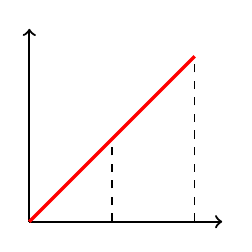
\begin{tikzpicture}[scale=0.7]
\draw[thick,->] (0,0)--(3.5,0);
\draw[thick,->] (0,0)--(0,3.5);
\draw[very thick, red] (0,0)--(3,3);
\draw[dashed] (3,0)--(3,3);
\draw[dashed] (1.5,0)--(1.5,1.5);
\end{tikzpicture}
\end{figure}

\section{Listings}

There are two basic forms of listings: the source code listings and the pseudocodes.
The first can be typeset using the \texttt{lstlisting} environment from the \texttt{listings} package,
which is included into the classfile and slightly tuned for you.
The example of the ``Hello, World!'' program in Java is given in Listing~\ref{lst1}.
An example of a very big listing spanning multiple pages is given in the appendix (Listing~\ref{lstX}).

\begin{lstlisting}[float=!h,caption={An example of the source code in Java},label={lst1}]
public class HelloWorld {
    public static void main(String[] args) {
        System.out.println("Hello, world!");
    }
}
\end{lstlisting}

The pseudocode can be typeset using a large variety of packages. This classfile has the \texttt{algorithmicx} package preconfigured.
As it does not generate floating environments on its own, the \texttt{algorithm} package is also included.
An example of them being used together is given in Listing~\ref{lst2}.

\begin{algorithm}[!h]
\caption{An example of the pseudocode}\label{lst2}
\begin{algorithmic}
	\Function{IsPrime}{$N$}
		\For{$t \gets [2; \lfloor\sqrt{N}\rfloor]$}
			\If{$N \bmod t = 0$}
				\State\Return \textsc{false}
			\EndIf
		\EndFor
		\State\Return \textsc{true}
	\EndFunction
\end{algorithmic}
\end{algorithm}

Just as a proof of concept, one can also float listings by \texttt{listings} using \texttt{algorithm},
of which an example is given in Listing~\ref{lst3}.

\begin{algorithm}[!h]
\caption{\texttt{listings} meet \texttt{algorithm}}\label{lst3}
\begin{lstlisting}
public class HelloWorld {
    public static void main(String[] args) {
        System.out.println("Hello, world!");
    }
}
\end{lstlisting}
\end{algorithm}

\chapter{Validation of float numbering}

Listing~\ref{lst4} shall have number~4.

\begin{algorithm}[!h]
\caption{\texttt{listings} meet \texttt{algorithm}}\label{lst4}
\begin{lstlisting}
public class HelloWorld {
    public static void main(String[] args) {
        System.out.println("Hello, world!");
    }
}
\end{lstlisting}
\end{algorithm}

Figure~\ref{fig2} shall have number~2.

\begin{figure}[!h]
\caption{An example of a figure}\label{fig2}
\centering
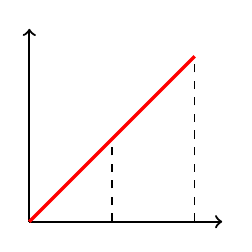
\begin{tikzpicture}[scale=0.7]
\draw[thick,->] (0,0)--(3.5,0);
\draw[thick,->] (0,0)--(0,3.5);
\draw[very thick, red] (0,0)--(3,3);
\draw[dashed] (3,0)--(3,3);
\draw[dashed] (1.5,0)--(1.5,1.5);
\end{tikzpicture}
\end{figure}

Table~\ref{tab3} shall have number~3.

\begin{table}[!h]
\caption{The multiplication table in \texttt{tabularx} (a fragment)}\label{tab3}
\centering
\begin{tabularx}{\textwidth}{|*{18}{>{\centering\arraybackslash}X|}}\hline
-- & 1 & 2 & 3 & 4 & 5 & 6 & 7 & 8 & 9 & 10 & 11 & 12 & 13 & 14 & 15 & 16 & 17 \\\hline
1  & 1 & 2 & 3 & 4 & 5 & 6 & 7 & 8 & 9 & 10 & 11 & 12 & 13 & 14 & 15 & 16 & 17 \\\hline
2  & 2 & 4 & 6 & 8 & 10 & 12 & 14 & 16 & 18 & 20 & 22 & 24 & 26 & 28 & 30 & 32 & 34 \\\hline
3  & 3 & 6 & 9 & 12 & 15 & 18 & 21 & 24 & 27 & 30 & 33 & 36 & 39 & 42 & 45 & 48 & 51 \\\hline
4  & 4 & 8 & 12 & 16 & 20 & 24 & 28 & 32 & 36 & 40 & 44 & 48 & 52 & 56 & 60 & 64 & 68 \\\hline
\end{tabularx}
\end{table}

\chapterconclusion

One shall typically make conclusions at the end of each chapter. From this chapter, we can conclude that
the numbering is correct, hooray!

\startconclusionpage

Here be the conclusion.

\printmainbibliography

\appendix

\chapter{An example of an appendix}\label{sec:app:1}

The appendices shall have all the floats numbered within each ``chapter''. Let's check it.

Listing~\ref{lst4:apx} shall have number~A.1.

\begin{algorithm}[!h]
\caption{\texttt{listings} meet \texttt{algorithm}}\label{lst4:apx}
\begin{lstlisting}
public class HelloWorld {
    public static void main(String[] args) {
        System.out.println("Hello, world!");
    }
}
\end{lstlisting}
\end{algorithm}

Figure~\ref{fig2:apx} shall have number~A.1.

\begin{figure}[!h]
\caption{An example of a figure}\label{fig2:apx}
\centering
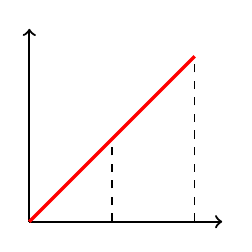
\begin{tikzpicture}[scale=0.7]
\draw[thick,->] (0,0)--(3.5,0);
\draw[thick,->] (0,0)--(0,3.5);
\draw[very thick, red] (0,0)--(3,3);
\draw[dashed] (3,0)--(3,3);
\draw[dashed] (1.5,0)--(1.5,1.5);
\end{tikzpicture}
\end{figure}

Table~\ref{tab3:apx} shall have number~A.1.

\begin{table}[!h]
\caption{The multiplication table in \texttt{tabularx} (a fragment)}\label{tab3:apx}
\centering
\begin{tabularx}{\textwidth}{|*{18}{>{\centering\arraybackslash}X|}}\hline
-- & 1 & 2 & 3 & 4 & 5 & 6 & 7 & 8 & 9 & 10 & 11 & 12 & 13 & 14 & 15 & 16 & 17 \\\hline
1  & 1 & 2 & 3 & 4 & 5 & 6 & 7 & 8 & 9 & 10 & 11 & 12 & 13 & 14 & 15 & 16 & 17 \\\hline
2  & 2 & 4 & 6 & 8 & 10 & 12 & 14 & 16 & 18 & 20 & 22 & 24 & 26 & 28 & 30 & 32 & 34 \\\hline
3  & 3 & 6 & 9 & 12 & 15 & 18 & 21 & 24 & 27 & 30 & 33 & 36 & 39 & 42 & 45 & 48 & 51 \\\hline
4  & 4 & 8 & 12 & 16 & 20 & 24 & 28 & 32 & 36 & 40 & 44 & 48 & 52 & 56 & 60 & 64 & 68 \\\hline
\end{tabularx}
\end{table}

Let's also check the enumerations. The unnumbered ones (the \texttt{itemize} environment):
\begin{itemize}
    \item item A;
    \item item B;
    \item item C;
\end{itemize}

The numbered ones.
\begin{enumerate}
    \item the first element;
    \item the second element, but we need to go deeper:
    \begin{enumerate}
        \item the first subelement;
        \item the second subelement;
        \item the third subelement;
    \end{enumerate}
    \item the third element;
    \item the fourth element;
    \item the fifth element (!);
    \item the sixth element;
    \item the seventh element;
    \item the eighth element;
    \item the ninth element;
    \item the tenth element.
\end{enumerate}

\chapter{Yet another example of an appendix, whose long title checks the requirement of GOST, which forbids hyphenation in the titles, as well as in the Table of Contents}\label{sec:app:2}

Let's check, using tables as an example, that floats in appendices are really numbered by ``chapters''.
Table~\ref{tab3:apx2} shall have number~B.1.

\begin{table}[!h]
\caption{The multiplication table in \texttt{tabularx} (a fragment)}\label{tab3:apx2}
\centering
\begin{tabularx}{\textwidth}{|*{18}{>{\centering\arraybackslash}X|}}\hline
-- & 1 & 2 & 3 & 4 & 5 & 6 & 7 & 8 & 9 & 10 & 11 & 12 & 13 & 14 & 15 & 16 & 17 \\\hline
1  & 1 & 2 & 3 & 4 & 5 & 6 & 7 & 8 & 9 & 10 & 11 & 12 & 13 & 14 & 15 & 16 & 17 \\\hline
2  & 2 & 4 & 6 & 8 & 10 & 12 & 14 & 16 & 18 & 20 & 22 & 24 & 26 & 28 & 30 & 32 & 34 \\\hline
3  & 3 & 6 & 9 & 12 & 15 & 18 & 21 & 24 & 27 & 30 & 33 & 36 & 39 & 42 & 45 & 48 & 51 \\\hline
4  & 4 & 8 & 12 & 16 & 20 & 24 & 28 & 32 & 36 & 40 & 44 & 48 & 52 & 56 & 60 & 64 & 68 \\\hline
\end{tabularx}
\end{table}

\chapter{An example of a large listing spanning multiple pages}

\begin{lstlisting}[caption={A very big listing},label={lstX}]
import java.util.*;

public class Example {
    static int[] restoreOutgoing(int[] g, int[] outgoing,
                                 int vertex, int mask) {
        int[] rv = new int[1 + Integer.bitCount(mask)];
        int n = g.length;
        int current = rv.length - 1;
        while (true) {
            rv[current] = vertex;
            if (current == 0) {
                if (vertex != 0) {
                    throw new AssertionError();
                }
                return rv;
            }
            mask ^= 1 << (vertex - 1);
            int prevMask = outgoing[mask] & g[vertex];
            if (prevMask == 0) {
                throw new AssertionError();
            }
            vertex = Integer.numberOfTrailingZeros(prevMask);
            --current;
        }
    }

    static int[] restoreIncoming(int[] g, int[] incoming,
                                 int vertex, int mask) {
        int[] rv = new int[1 + Integer.bitCount(mask)];
        int n = g.length;
        int current = 0;
        while (true) {
            rv[current] = vertex;
            if (current == rv.length - 1) {
                if (vertex != 0) {
                    throw new AssertionError();
                }
                return rv;
            }
            mask ^= 1 << (vertex - 1);
            int nextMask = incoming[mask] & g[vertex];
            if (nextMask == 0) {
                throw new AssertionError();
            }
            vertex = Integer.numberOfTrailingZeros(nextMask);
            ++current;
        }
    }
}
\end{lstlisting}
                
\end{document}
